\documentclass{article}

\usepackage[colorlinks]{hyperref}
\usepackage{booktabs}
\usepackage{graphicx}

\usepackage[many]{tcolorbox}

% https://tex.stackexchange.com/questions/181082/how-to-reproduce-this-box-in-tcolorbox
\newtcbox{\srcbox}{
  enhanced,
  nobeforeafter,
  tcbox raise base,
  boxrule=0.4pt,
  top=0mm,
  bottom=0mm,
  right=0mm,
  left=4mm,
  arc=1pt,
  boxsep=2pt,
  before upper={\vphantom{dlg}},
  colframe=teal!75!white,
  coltext=teal!25!black,
  colback=teal!5!white,
  overlay={
    \begin{tcbclipinterior}
      \fill[teal!75!white] (frame.south west) rectangle node[text=white,font=\sffamily\bfseries\tiny,rotate=90] {SRC} ([xshift=4mm]frame.north west);
    \end{tcbclipinterior}
  }
}

\newtcolorbox{featurebox}[1]{colback=teal!5!white,colframe=teal!75!white,title={#1}}

\newtcolorbox{codebox}{colback=teal!5!white,colframe=teal!75!white}


\newcommand{\caper}{\textsc{Capernaum}}
\newcommand{\cfse}{\textsc{C4se}}
\newcommand{\cls}{\textsc{Cls}}
\newcommand{\ghsrc}[2]{\href{https://github.com/quantum-bits/capernaum/blob/development/#1}{#2}}
\newcommand{\gql}{\textsc{GraphQL}}
\newcommand{\pg}{\textsc{PostgreSQL}}

\title{\caper{} Architecture}
\author{Dr.\ Tom Nurkkala}

\begin{document}
\maketitle

\begin{cbox}{Features}
  \begin{enumerate}
  \item \gql{} API
  \item Fully-open source on \href{https://github.com/quantum-bits/capernaum.git}{GitHub}
  \end{enumerate}
\end{cbox}

\section{Introduction}
\label{sec:introduction}

\caper{} is a web-based system
that gathers respones to designated surveys taken at \href{https://www.qualtrics.com/}{Qualtrics}.
When notified of a completed survey by a Qualtrics web hook,
\caper{}
downloads the survey response
to its \href{https://www.postgresql.org/}{\pg{}} relational database
using the
\href{https://api.qualtrics.com/}{Qualtrics RESTful API}.
\caper{} then
analyzes the response and
prepares a personalized analysis for the respondent:
a \LaTeX-formatted PDF containing both a text commentary
and graphical visualizations of results.
Finally, \caper{}
emails the PDF to the survey respondent.

The main customer for \caper{}
is Taylor University's
\href{https://www.taylor.edu/center-for-scripture-engagement/}{Center for Scripture Engagement}
(\cfse).
As part of a faith-based institution,
the \cfse{} publishes the
\href{https://www.taylor.edu/center-for-scripture-engagement/survey/}{Christian Life Survey}
(\cls)
at Qualtrics.
\caper{} provides analysis and reporting on survey results
for individual respondents and
can also aggregate responses for groups of users.

Traffic to the \cls{} is driven primarily by a partnership between \cfse{} and
\href{https://www.biblegateway.com/}{Bible Gateway}.
Bible Gateway is one of the most-visited Christian web site on the Internet.
In October, 2021, it was the
\href{https://www.similarweb.com/website/biblegateway.com/}{632-nd most visited site in the world,
  with 80~million visits}.
Although only a fraction of Bible Gateway users take the \cls,
the potential user volume is a key factor in the design of \caper.
In particular, \caper{} employs a distributed job queuing system
for analysis and production of survey analyses,
designed to scale to handle 2,000 survey responses per minute.

\begin{figure}
  \centering
  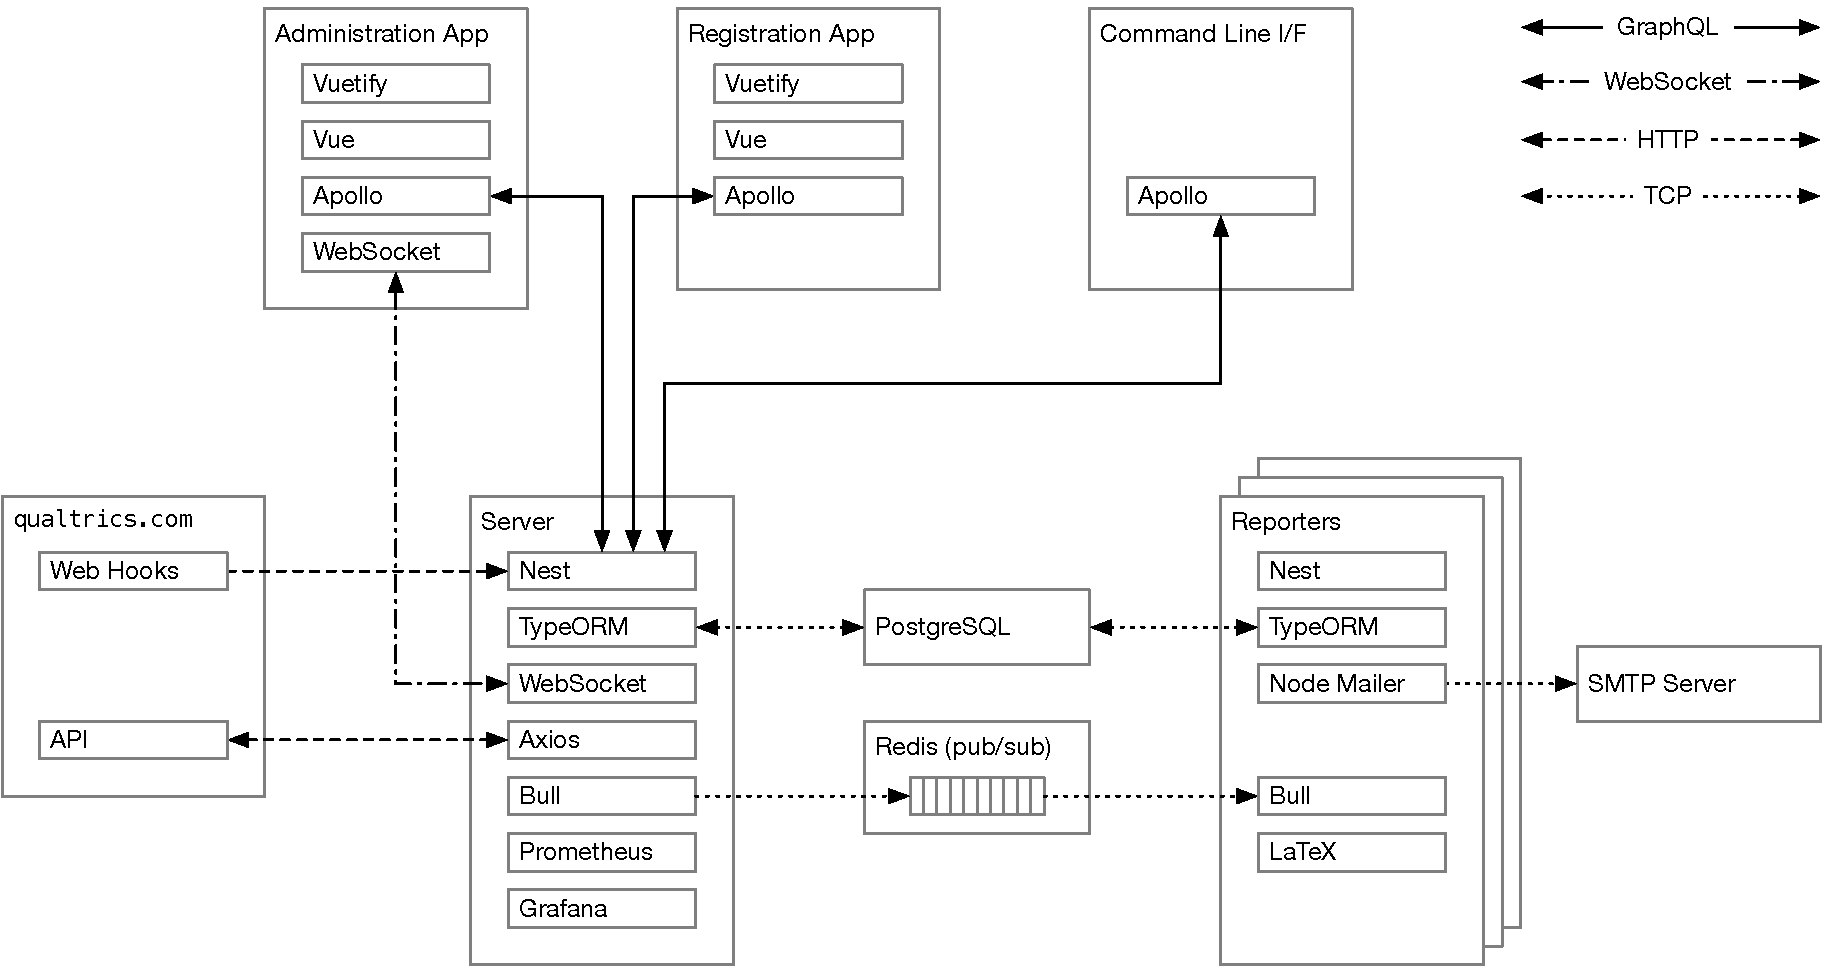
\includegraphics[width=\textwidth]{block-diagram}
  \caption{Block diagram of \caper.
    Communication between distributed processes is indicated in the legend.}
  \label{fig:block-diagram}
\end{figure}

\section{Deployment}
\label{sec:deployment}

\caper{} employs a fully-automated deployment
using \href{https://www.ansible.com/}{Ansible}.
The \ghsrc{ansible/provision.yaml}{provisioning file} contains commands for GitHub, OS updates, etc.

\end{document}

%%% Local Variables:
%%% mode: latex
%%% TeX-master: t
%%% End:

% LocalWords:  Ansible ansible
